\clearpage
\noindent
\begin{center}
    \Large \textbf{Appendix}
\end{center}
\vspace{-1em} % 可调节，让标题更贴顶


\section{The Use of Large Language Models (LLMs)}

\begin{algorithm}[h]
\caption{Keyframe Extraction via Bidirectional CLIP Similarity}
\begin{algorithmic}[1]
\REQUIRE Video frame sequence \texttt{frames}, similarity thresholds $t_1$ (scene change) and $t_2$ (diversity)
\ENSURE Selected keyframe indices \texttt{sel}
\STATE Initialize \texttt{sel} with the first frame index: \texttt{sel} $\leftarrow \{0\}$
\STATE Extract CLIP feature for the first frame: \texttt{prev} $\leftarrow$ clip(\texttt{frames}[0])
\FOR{each frame $c$ in \texttt{frames[1:]} with index $i$}
    \STATE \texttt{curr} $\leftarrow$ clip($c$)
    \STATE $s \leftarrow$ sim(\texttt{curr}, \texttt{prev})
    \IF{$s < t_1$}
        \FOR{each future frame $f$ in \texttt{frames}[$i+1$ : ]}
            \STATE \texttt{fut} $\leftarrow$ clip($f$)
            \IF{sim(\texttt{curr}, \texttt{fut}) $< t_2$}
                \STATE Add index $i$ to \texttt{sel}
                \STATE \texttt{prev} $\leftarrow$ \texttt{curr}
                \STATE \textbf{break}
            \ENDIF
        \ENDFOR
    \ENDIF
\ENDFOR
\IF{sim(clip(\texttt{frames}[-1]), \texttt{prev}) $< t_1$}
    \STATE Add last frame index to \texttt{sel}
\ENDIF
\RETURN \texttt{sel}
\end{algorithmic}
\label{alg:keyframe_clip}
\end{algorithm}

In this work, Large Language Models (LLMs) were employed in four main ways: (i) to aid and polish the writing for clarity and style; and (ii) to provide coding assistance, including code generation, debugging, and optimization suggestions.

Specifically, LLMs were utilized to improve the clarity, coherence, and readability of the manuscript, with particular attention given to the \textbf{Related Work}, \textbf{Method}, and \textbf{Experiments} sections. In these parts, the initial drafts were carefully reviewed and refined using LLM-powered suggestions for sentence structure, terminology, and logical flow. This process ensured that the technical content was presented in a precise and accessible manner, while maintaining consistency in academic tone and style throughout the paper.

All outputs generated by LLMs were critically reviewed, verified, and further refined by the authors. The core scientific ideas, methodology, and contributions remain entirely the authors’ own. The use of LLMs was strictly limited to language enhancement and coding support, without influencing the originality or integrity of the research.

\section{Inference time}
In Table~\ref{tab:table1}, we evaluated the speed of our model on a single NVIDIA A100 GPU. We employed LLaVA-Video-7B~\cite{zhang2024video} as our answering LLM, implemented a 32-frame sampling strategy from 512 input frames in total, and generated 27 text tokens. Additionally, we leveraged KV Cache and Flash Attention~\cite{dao2022flashattention, dao2023flashattention2} to enhance inference efficiency.

Our detailed analysis of computational costs reveals that processing each video sample requires a total of $6.42$ seconds, with the Vision Encoder ($2.92$ seconds) and LLM ($2.89$ seconds) dominating the time consumption. These two components collectively consume $90\%$ of the total processing time, indicating the direction for future system optimization. In contrast, our VideoITG module demonstrates remarkable efficiency, requiring only $0.61$ seconds to scan $512$ frames—a speed that surpasses human visual recognition and thinking capabilities.

\begin{table}[ht]
  \centering
  \setlength{\tabcolsep}{1.5mm}{
  \caption{Computation cost of the model.}\vspace{2mm}
  \label{tab:table1}
  \begin{tabular}{c c c c c c}
  \toprule
   Vision Encoder & VideoITG & LLM & Overall \\
  \midrule
   2.92s & 0.61s & 2.89s & 6.42s  \\
  \bottomrule
  \end{tabular}
  } 
\end{table}

\begin{table*}[!h]
\centering
\caption{The performance (accuracy) of SOTA methods on video benchmarks. For InternVL2.5-8B results, we report the higher results in the technical report and lmms-eval. We sample 32 frames using VideoITG for our results.}\vspace{1mm}
\label{tab:video-bench}
\renewcommand{\arraystretch}{0.9}
\small
\resizebox{\textwidth}{!}{
\setlength{\tabcolsep}{1pt}
\begin{tabular}{@{}lc|ccccccc@{}}
    \toprule
     & \multicolumn{1}{c|}{\scriptsize{\textbf{Open-Ended Q\&A}}} & \multicolumn{7}{c}{\scriptsize{\textbf{Multi-Choice Q\&A}}}  \\   
    \multirow{2}{*}{\textbf{Model}} & \rotatebox{45}{\textbf{\scriptsize{ActNet-QA}}} & \rotatebox{45}{\textbf{\scriptsize{EgoSchema}}} & \rotatebox{45}{\textbf{\scriptsize{MLVU}}} & \rotatebox{45}{\textbf{\scriptsize{NExT-QA}}} & \rotatebox{45}{\textbf{\scriptsize{PerceptionTest}}}  & \rotatebox{45}{\textbf{\scriptsize{LongVideoBench}}} &\rotatebox{45}{\textbf{\scriptsize{VideoMME}}} &\rotatebox{45}{\textbf{\scriptsize{MVBench}}} \\ \cmidrule(l){2-9} 
    & test & test & m-avg & mc & val   & val & wo/w-subs & val \\ \midrule
    \multicolumn{9}{l}{\textit{Open-source models}} \\
    VILA-40B~\cite{lin2024vila} & 58.0 & 58.0 & - & 67.9 & 54.0  & -  & 60.1/61.1 & - \\
    PLLaVA-34B~\cite{xu2024pllava} & 60.9 & - & - & - & - & 53.2 & - & 58.1 \\    
    VideoLLaMA2-7B~\cite{cheng2024videollama} & 50.2 & 50.5 & - & - & 49.6 & - & 45.1/46.6 & 53.4 \\ 
    LongVA-7B~\cite{zhang2024long} & 50.0 & - & 56.3 & 68.3 & -  & -  & 52.6/54.3 & - \\ 
    LongVU-7B~\cite{zhang2024long} & - & 67.6 & 65.4 & - & -  & -  & 60.6/- & 66.9 \\
    LLaVA-OV-7B~\cite{li2024llavaonevision} & 56.6 & 60.1 & 64.7 & 79.4 & 57.1    & 56.5 & 58.2/61.5 & 56.7 \\
    mPLUG-Owl3-8B~\cite{ye2024mplug} & - & - & - & 78.6 & - & 52.1 & 53.5/- & 54.5 \\ 
    LLaVA-Video-7B~\cite{zhang2024video} & 56.5 & 57.3 & 70.8 & 83.2 & 67.9 & 58.2 & 63.3/69.7 & 58.6 \\
    Qwen2.5-VL-7B~\cite{wang2024qwen2} & - & - & - & 70.2 & 70.5 & 54.7 & 65.1/71.6 & 69.6 \\
    InternVL2.5-8B~\cite{zhang2024internlm} & - & 51.5 & 68.9 & - & - & 60.0 & 64.2/66.9 & 72.0 \\
    \midrule 
    \rowcolor[HTML]{DAEFF9}
    InternVL2.5-8B-ITG-32 & 57.4 & 51.6  & 75.0 & 79.5 & 64.9 & 61.9 & 67.3/69.6 & 72.2 \\ 
    \bottomrule
    \end{tabular}
}
\end{table*}


\begin{table*}[t]
\centering
\caption{Dataset quality (IoU). We evaluate the performance in both multiple-choice (MC) and open-ended (OE) questions.}
\label{tab:ablate_dataset}\vspace{2mm}
\resizebox{0.99\textwidth}{!}{
\setlength{\tabcolsep}{3.5pt}
\begin{tabular}{c|cccc}  %  c c
\toprule
\textbf{Method} & \textbf{Semantic-MC} & \textbf{Semantic \& Motion-OE} & \textbf{Semantic-MC} & \textbf{Semantic \& Motion-OE}  \\
\midrule
Qwen2.5-VL-32B & 0.31 & 0.36 & 0.27 & 0.37 \\
GPT4o & 0.24 & 0.30 & 0.26 & 0.27 \\
Ours & \textbf{0.79} & \textbf{0.74} & \textbf{0.72} & \textbf{0.69} \\
\bottomrule
\end{tabular}
}
\end{table*}

\section{Dataset details}
\subsection{Prompt template}
Our Question-guided Clip Retrieval process utilizes a carefully designed prompt template (shown in Table~\ref{tab:temporal_grounding_prompt}) that instructs the LLM to analyze chronologically ordered clip-level descriptions and identify the minimal set of clips necessary to answer a given question.
The prompt template consists of three main components:

\begin{itemize}[leftmargin=6mm]
    \item \textbf{Task Description}: Defines the LLM's role as an expert in analyzing video clip descriptions and establishes the goal of selecting clips that cover both question and answer content.
    \item \textbf{Guidelines}: Provides detailed instructions for clip selection, including handling time-related expressions, determining if a single or multiple clips are needed, addressing questions about object existence or movement, and avoiding unnecessary clips.
    \item \textbf{Output Format}: Specifies the required JSON structure for responses, ensuring consistent formatting with explanation and clip number fields.
\end{itemize}

This template enables the LLM to perform chain-of-thought reasoning when selecting relevant clips. The model analyzes keywords from questions, identifies temporal relationships (\eg, ``before," ``after"), and provides explicit rationales for its selections. For cases where no relevant clips exist, the model returns ``None" to reduce annotation noise.

\begin{table*}[t!]\centering
\caption{Prompt Template: An expert system for temporal localization in video segments. The system analyzes video segment descriptions to determine the minimal and necessary combination of segments required to answer questions.}
\label{tab:temporal_grounding_prompt}\vspace{2mm}
\begin{minipage}{\linewidth}
\centering
\begin{tcolorbox} 
\centering
\footnotesize
\begin{tabular}{p{0.9\columnwidth} c}
\normalsize\color{blue}{\textbf{Task:}} &\\
You are an expert in analyzing video clip descriptions. Your task is to select which clip or combination of clips is necessary to answer the given question, ensuring the selected clips effectively cover the content of both the question and the answer. & \\
\midrule
\normalsize\color{blue}{\textbf{Guidelines:}} & \\
\begin{itemize}[leftmargin=6mm]
\item Carefully read the descriptions to determine which clip(s) provide relevant content for the question and the answer.
\item Clip descriptions are in chronological order. Use clip number to locate clips based on time-related expressions (e.g., "at the beginning of the video" suggests a smaller clip number, while "at the end of the video" suggests a larger one).
\item First, determine if one clip can answer the question or if multiple clips are needed. Then, return a list containing the selected clip(s) and an explanation.
\item If the question asks about the existence/movement of an object or event. The object/action/movement may not exist, meaning you can't find the answer in the description, but the question might still provide some clues. You need to find the sentence closest to those clues.
\item If asked about the whole video description or overall atmosphere, you should return all clip numbers.
\item If multiple clips provide similar descriptions of the content and any of them can be used to answer the question, return all corresponding clips.
\item If there are no clues in all descriptions and cannot answer the question, return "None.".
\item \textbf{Important}: Avoid including unnecessary clips.
\end{itemize} \\
\midrule

\normalsize\color{blue}{\textbf{Output Format:}} & \\
1. Your output should be formed in a JSON file. \\
2. Only return the Python dictionary string. \\
For example: \\
{\small\bfseries\texttt{\{"explanation": "...", "clip\_num": "One clip: [Clip-2]"\}}} \\
{\small\bfseries\texttt{\{"explanation": "...", "clip\_num": "Multiple clips: [Clip-1, Clip-7, Clip-8]"\}}} \\
{\small\bfseries\texttt{\{"explanation": "...", "clip\_num": "None."\}}} \\
    \end{tabular}
\end{tcolorbox}
\vspace{-2mm}
\end{minipage}
\end{table*}

\begin{table*}[t!]\centering
\caption{Prompt template for identifying motion-related questions in video QA tasks. The template instructs the system to analyze each question-answer pair and determine whether the question pertains to absolute or relative speed, responding with ``Yes'' or ``No'' accordingly. Example cases are provided for clarification.}
\label{tab:temporal_grounding_prompt_v1}\vspace{2mm}
\begin{minipage}{\linewidth}
\centering
\begin{tcolorbox} 
\centering
\footnotesize
\begin{tabular}{p{0.9\columnwidth} c}
\normalsize\color{blue}{\textbf{Task:}} &\\
Analyze the given QA pair to determine if the question is related to speed. Specifically, check if it involves either absolute speed (the speed of a specific object) or relative speed (comparing the speed of different objects). Provide an output of "Yes" if the question pertains to speed, and "No" otherwise. & \\
\textbf{Important}: Respond with "Yes" or "No" only.  & \\
\midrule
\normalsize\color{blue}{\textbf{Example:}} & \\
\textbf{Question 1:} Which is faster, the white car or the bicycle? Options: 
A. The bicycle. 
B. The white car. 
C. Both are at the same speed. 
D. None of the above. \\
\textbf{Answer 1:} B. The white car. \\
\textbf{Output:} Yes. \\
\textbf{Question 2:} What color is the cat ?Options: 
A. black 
B. white 
C. orange 
D. gray  \\
\textbf{Answer 2:} C. orange  \\
\textbf{Output:} No. \\
    \end{tabular}
\end{tcolorbox}
\vspace{-2mm}
\end{minipage}
\end{table*}

\begin{table*}[t!]\centering
\caption{Prompt template for identifying semantic-related questions in video QA tasks. The template instructs the system to analyze each question-answer pair and determine whether the question pertains to absolute or relative speed, responding with ``Yes'' or ``No'' accordingly. Example cases are provided for clarification.}
\label{tab:temporal_grounding_prompt_v2}\vspace{2mm}
\begin{minipage}{\linewidth}\vspace{0mm}
\centering
\begin{tcolorbox} 
\centering
\footnotesize
\begin{tabular}{p{0.9\columnwidth} c}
\normalsize\color{blue}{\textbf{Task:}} &\\
Analyze the given QA pair to determine if the question inquires about the existence of an object or action. If it does, and the answer is "No" (indicating non-existence), output "Yes." If the question is not about existence, or the answer is "Yes" (indicating existence), output "No."  & \\
\textbf{Important}: Respond with "Yes" or "No" only.  & \\
\midrule
\normalsize\color{blue}{\textbf{Example:}} & \\
\textbf{Question 1:} After going through the bag, does the person meticulously clean the area around the sink?  \\
\textbf{Answer 1:} No, the person does not clean the area around the sink after going through the bag. The video primarily focuses on the action of the person with the bag and items, not on cleaning activities. \\
\textbf{Output:} Yes. \\
\textbf{Question 2:} Is there a cat sitting on the windowsill in the video?  \\
\textbf{Answer 2:} Yes, there is a cat sitting on the windowsill throughout the video. \\
\textbf{Output:} No. \\
\midrule

\end{tabular}
\end{tcolorbox}
\vspace{-2mm}
\end{minipage}
\end{table*}



We implement this process using GPT-4o-mini~\cite{openai2024gpt4o}, which is sufficient for accurate clip selection while reducing annotation costs by over 10 times compared to larger models. The selected clips are then converted to event boundaries defined by timestamps based on frame indices for the final temporal grounding annotations.


\subsection{Human-in-the-loop verification}

Ensuring the quality of automatically annotated datasets is critical for the reliability and effectiveness of downstream video understanding models. In this work, we implement a comprehensive quality control protocol for the VideoITG-40K dataset.

Our pipeline begins with diverse sampling: we select a representative subset of the dataset, covering a wide range of instructions and video scenarios. For this subset, we conduct human verification, where expert annotators review the automatically generated annotations to assess their accuracy and relevance. This process allows us to identify and correct potential errors, and to further calibrate our annotation pipeline for improved consistency and quality.

As shown in Table~\ref{tab:ablate_dataset}, we compare our pipeline with baselines where advanced models such as Qwen2.5VL and GPT-4o are directly prompted to answer the temporal boundaries of relevant events. These direct approaches result in significantly lower performance, highlighting the advantage of our multi-step, instruction-guided annotation strategy.




\subsection{Frame Sampling Algorithm}
The algorithm in ~\ref{alg:keyframe_clip} is designed for semantic-only keyframe selection, aiming to extract a diverse set of frames that comprehensively capture the semantic content of a video—such as people, scenes, or objects. By leveraging CLIP features, the algorithm compares each frame to previously selected keyframes using a bidirectional similarity measure. Frames are selected when their semantic features differ significantly from both the last keyframe (scene change threshold) and from future frames (diversity threshold), ensuring that each chosen frame represents distinct semantic information. This process produces a set of keyframes with maximal semantic coverage and minimal redundancy, aligning with the goal of representing all major semantic aspects of the video.




\section{Visualization}
In Fig.~\ref{vis_a1} and Fig.~\ref{vis_a2}, 
we present two sets of results comparing sampling results of VideoITG with uniform sampling. Fig.~\ref{vis_a1} demonstrates a temporal reasoning problem, where our model accurately identifies the ``workout'' mentioned in the question and successfully locates the subsequent actions in the video, leading to the correct answer selection. In contrast, the uniform sampling strategy failed to capture these crucial frames. 
Fig.~\ref{vis_a2} illustrates a non-existence question scenario where our model effectively identifies all IMAX movies present in the given options, enabling it to successfully filter out and determine the correct answer.

\clearpage
\begin{figure*}[ht]
\centering
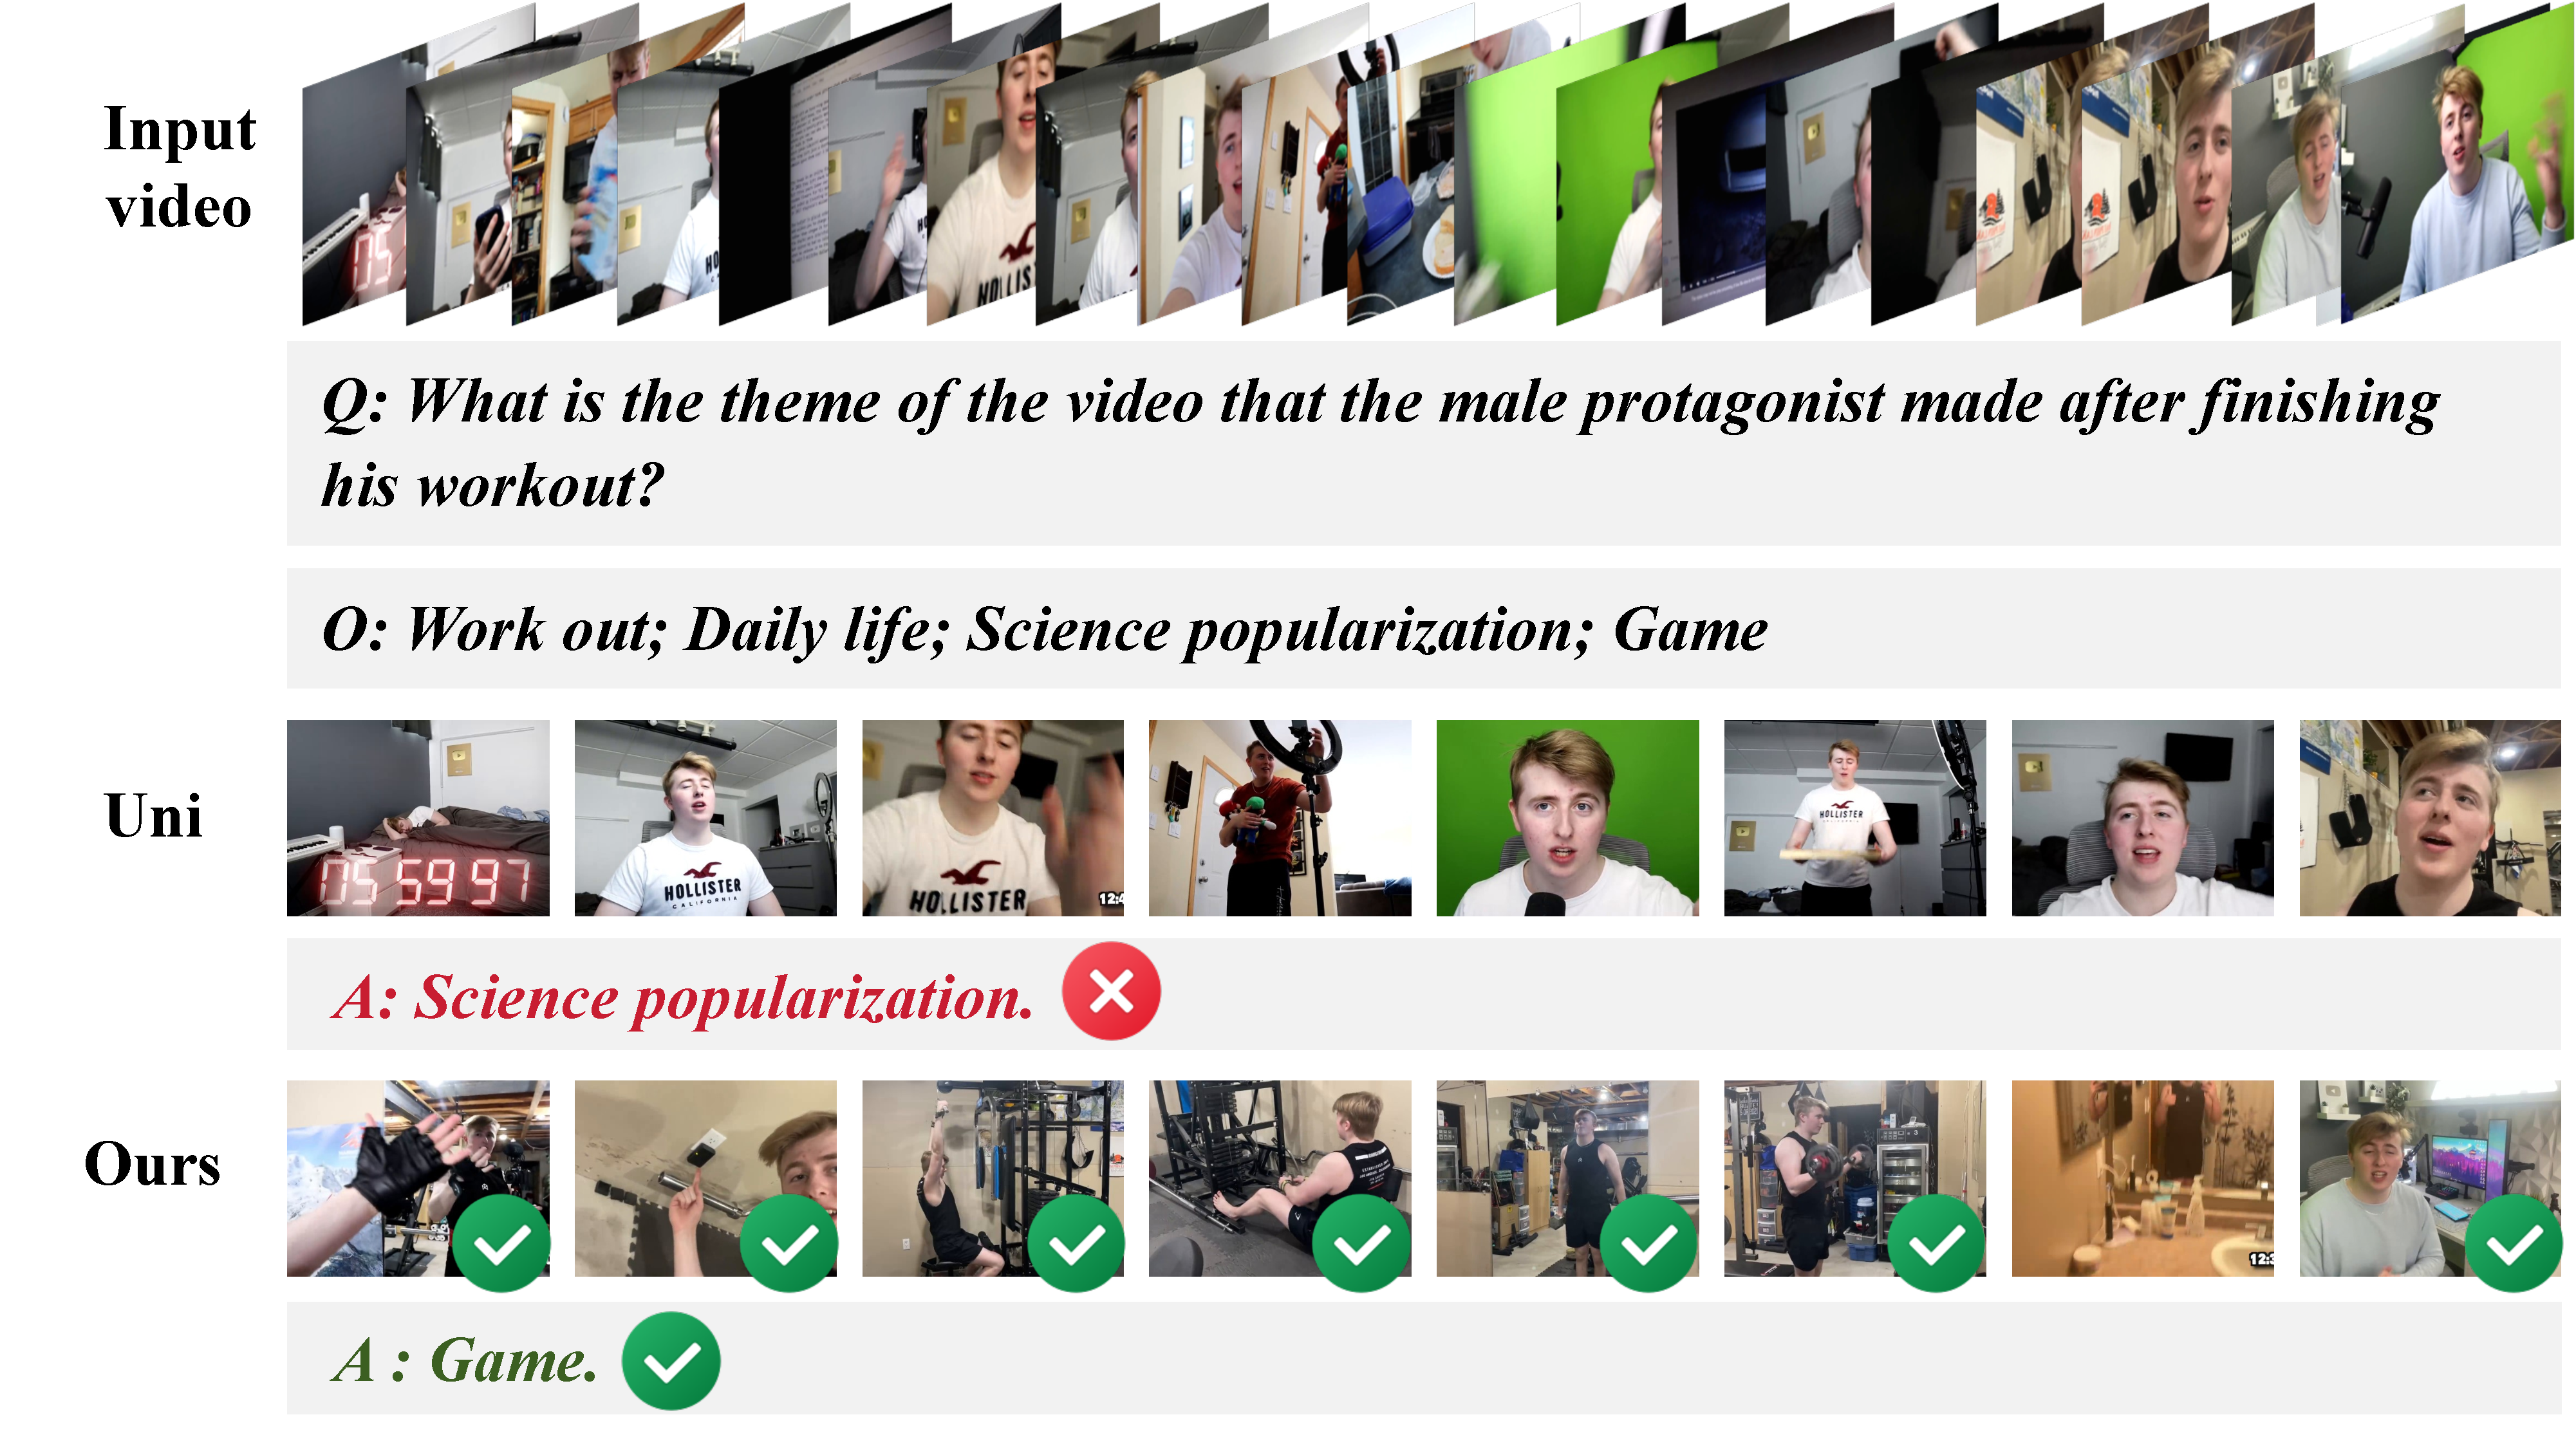
\includegraphics[width=\linewidth]{appendix_vis1.pdf}
\caption{Example-1 shows how different sampling strategies impact video understanding. We mark the identified key frames that directly answer the question with green check-marks.}
\label{vis_a1}
\end{figure*}

\begin{figure*}[!htbp]
\centering
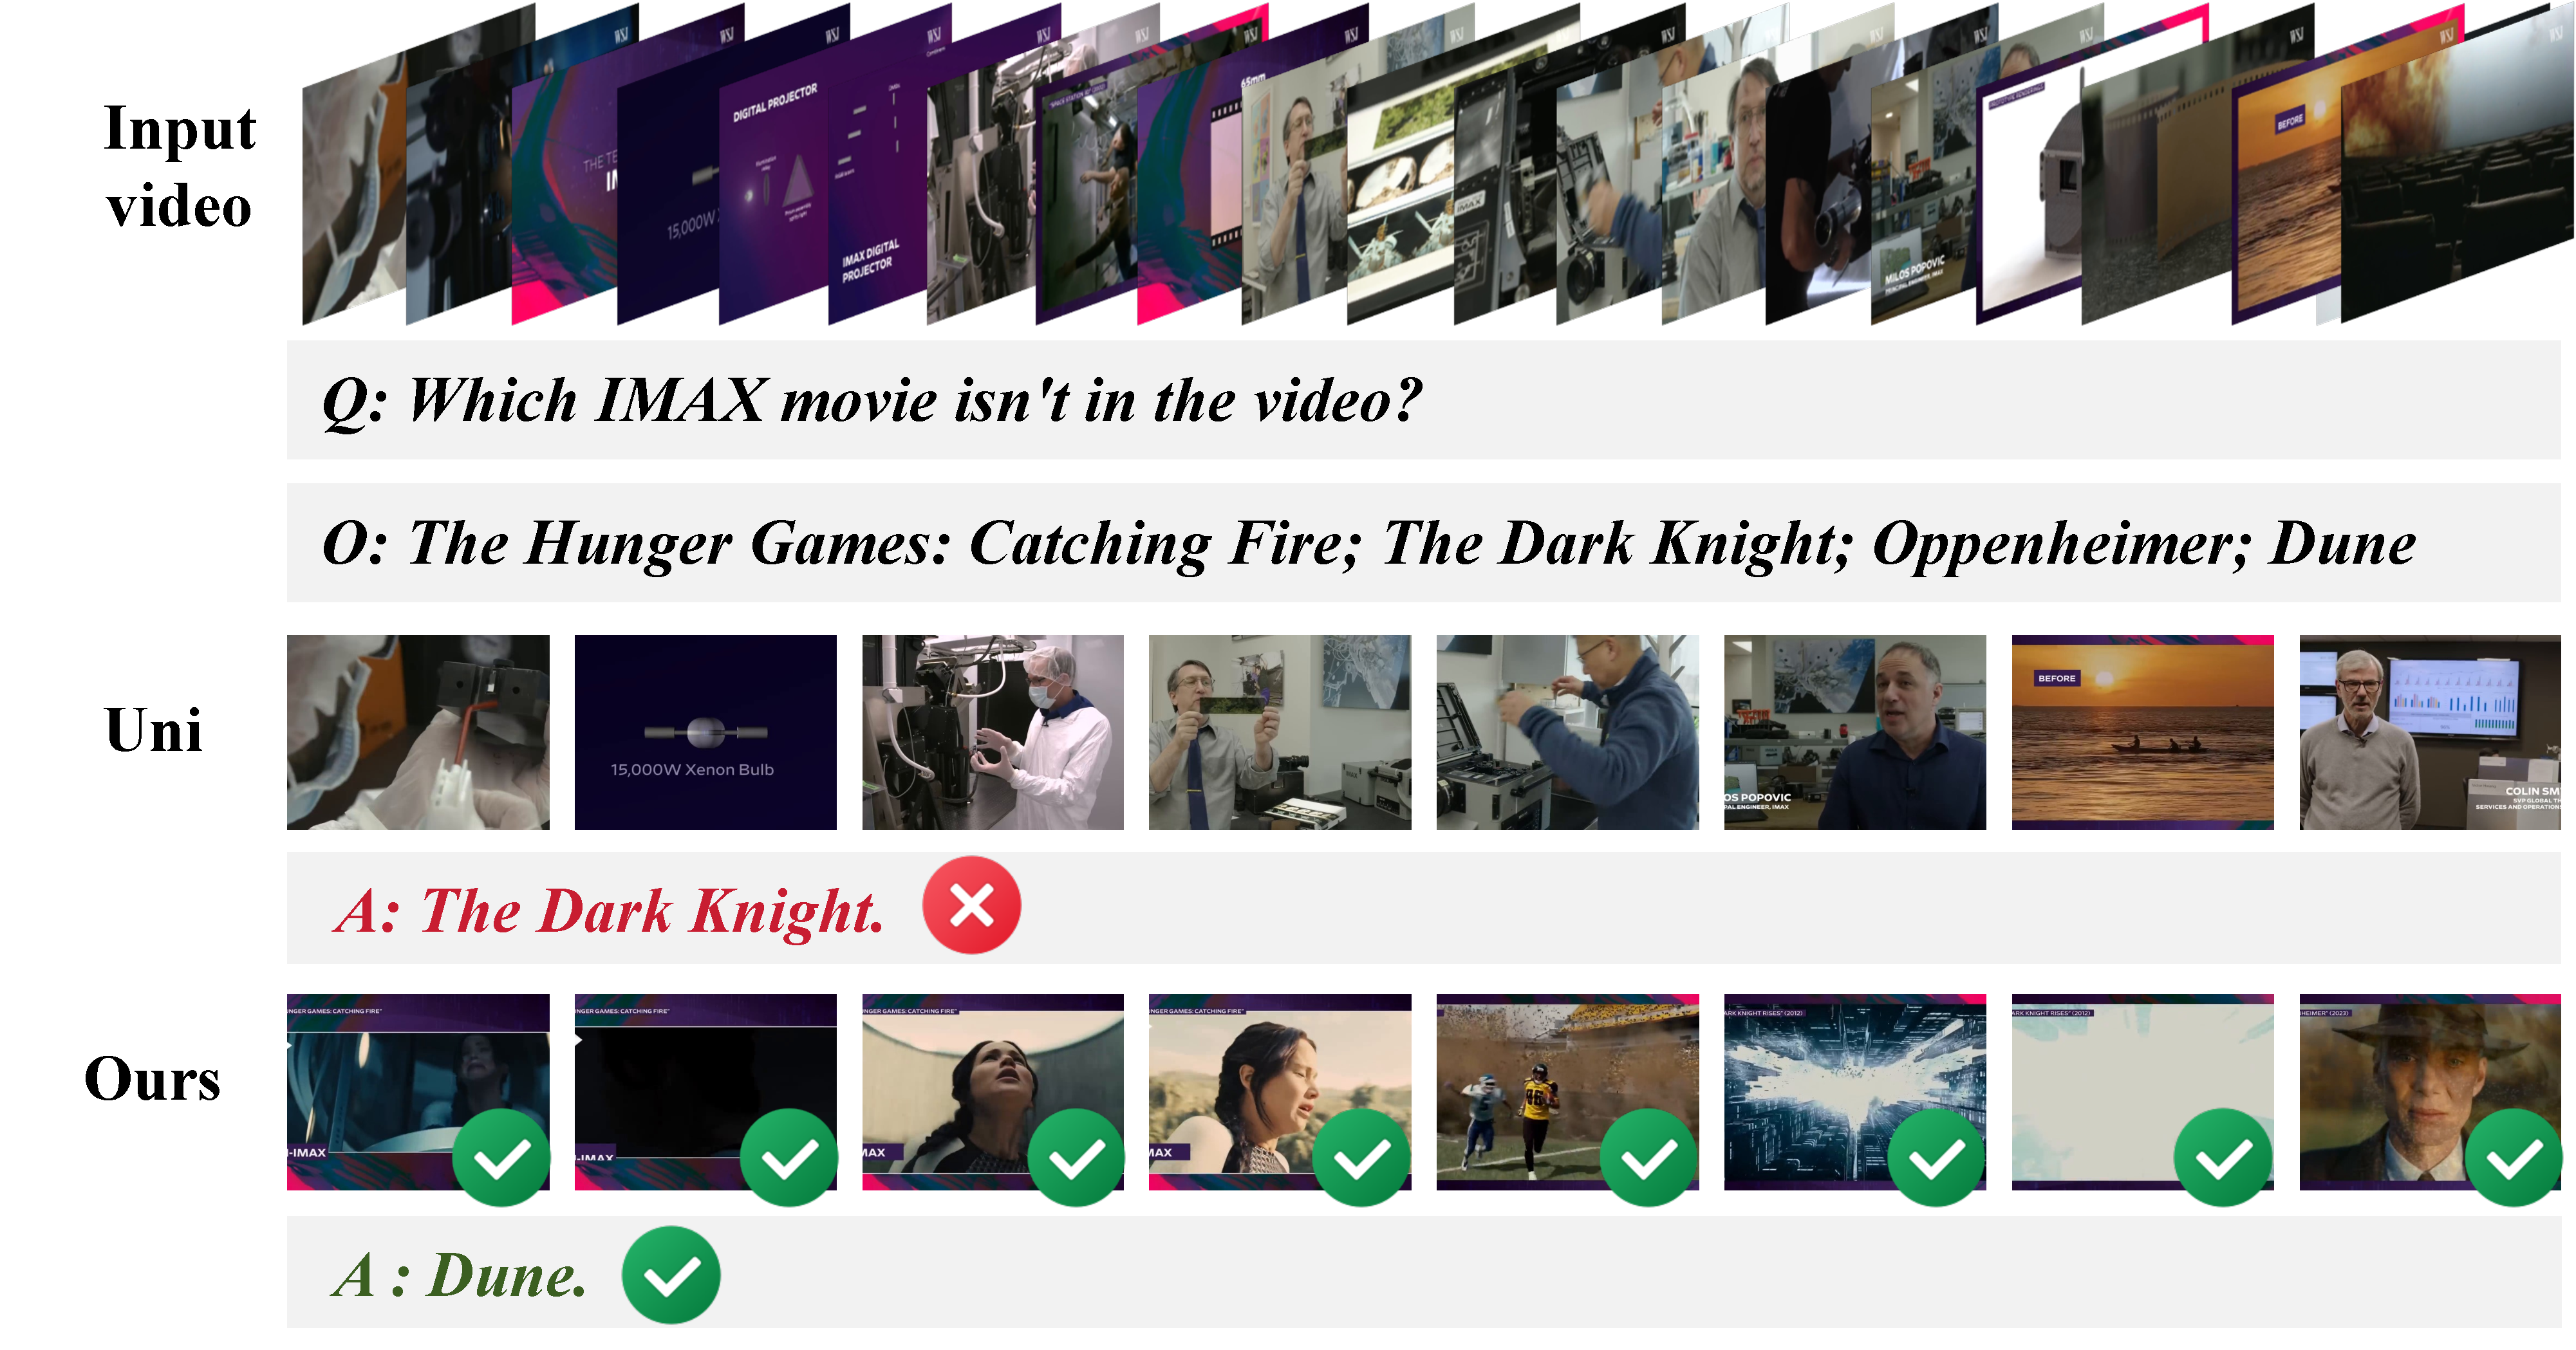
\includegraphics[width=\linewidth]{appendix_vis2.pdf}
\caption{Example-2 shows how different sampling strategies impact video understanding. We mark the identified key frames that directly answer the question with green check-marks.}
\label{vis_a2}
\end{figure*}